\section{STFT \& Spectrograms}
\begin{frame}{}
    \LARGE \textbf{STFT \& Spectrograms}
\end{frame}

\subsection{Fourier Transforms}
\begin{frame}[allowframebreaks]{Fourier Transforms You'll Actually Use}
    \begin{itemize}
        \item \textbf{Discrete Fourier Transform (DFT)}: A mathematical operation that converts a signal from the time domain to the frequency domain. It transforms $N$ samples of a discrete signal, $x[n]$, into $N$ frequency bins, $X[k]$. The formula for the DFT is:
        $$X[k] = \sum_{n=0}^{N-1} x[n]\,e^{-j2\pi kn/N}$$
        where $x[n]$ is the signal in the time domain, $X[k]$ is the signal in the frequency domain, $N$ is the total number of samples, $n$ is the sample index, and $k$ is the frequency bin index.
        \item \textbf{Fast Fourier Transform (FFT)}: This is not a different transform, but rather a computationally efficient algorithm for calculating the DFT.
    \end{itemize}
\framebreak
    To apply the Fourier transform in practice, you typically:
    \begin{enumerate}
        \item \textbf{Choose a window length ($N$)}: This determines the number of samples to be transformed at a time.
        \item \textbf{Choose a hop size}: This is the number of samples to advance before taking the next window.
    \end{enumerate}
    This process involves a fundamental trade-off: a longer window ($N$) provides better \textbf{frequency resolution} (ability to distinguish between close frequencies) but worse \textbf{time resolution} (ability to pinpoint when an event occurred). 
    
    Conversely, a shorter window improves time resolution at the expense of frequency resolution.

\framebreak

    We use Fourier transforms to analyze the frequency content of signals. The resulting frequency information (spectra) is essential for:
    
    \begin{itemize}
        \item \textbf{Building Spectrograms}: Visual representations of how the frequency content of a signal changes over time.
        \item \textbf{Extracting Features}: Deriving key characteristics from a signal that can be used for tasks like speech recognition, music information retrieval, and audio classification.
    \end{itemize}

    \begin{figure}
        \centering
        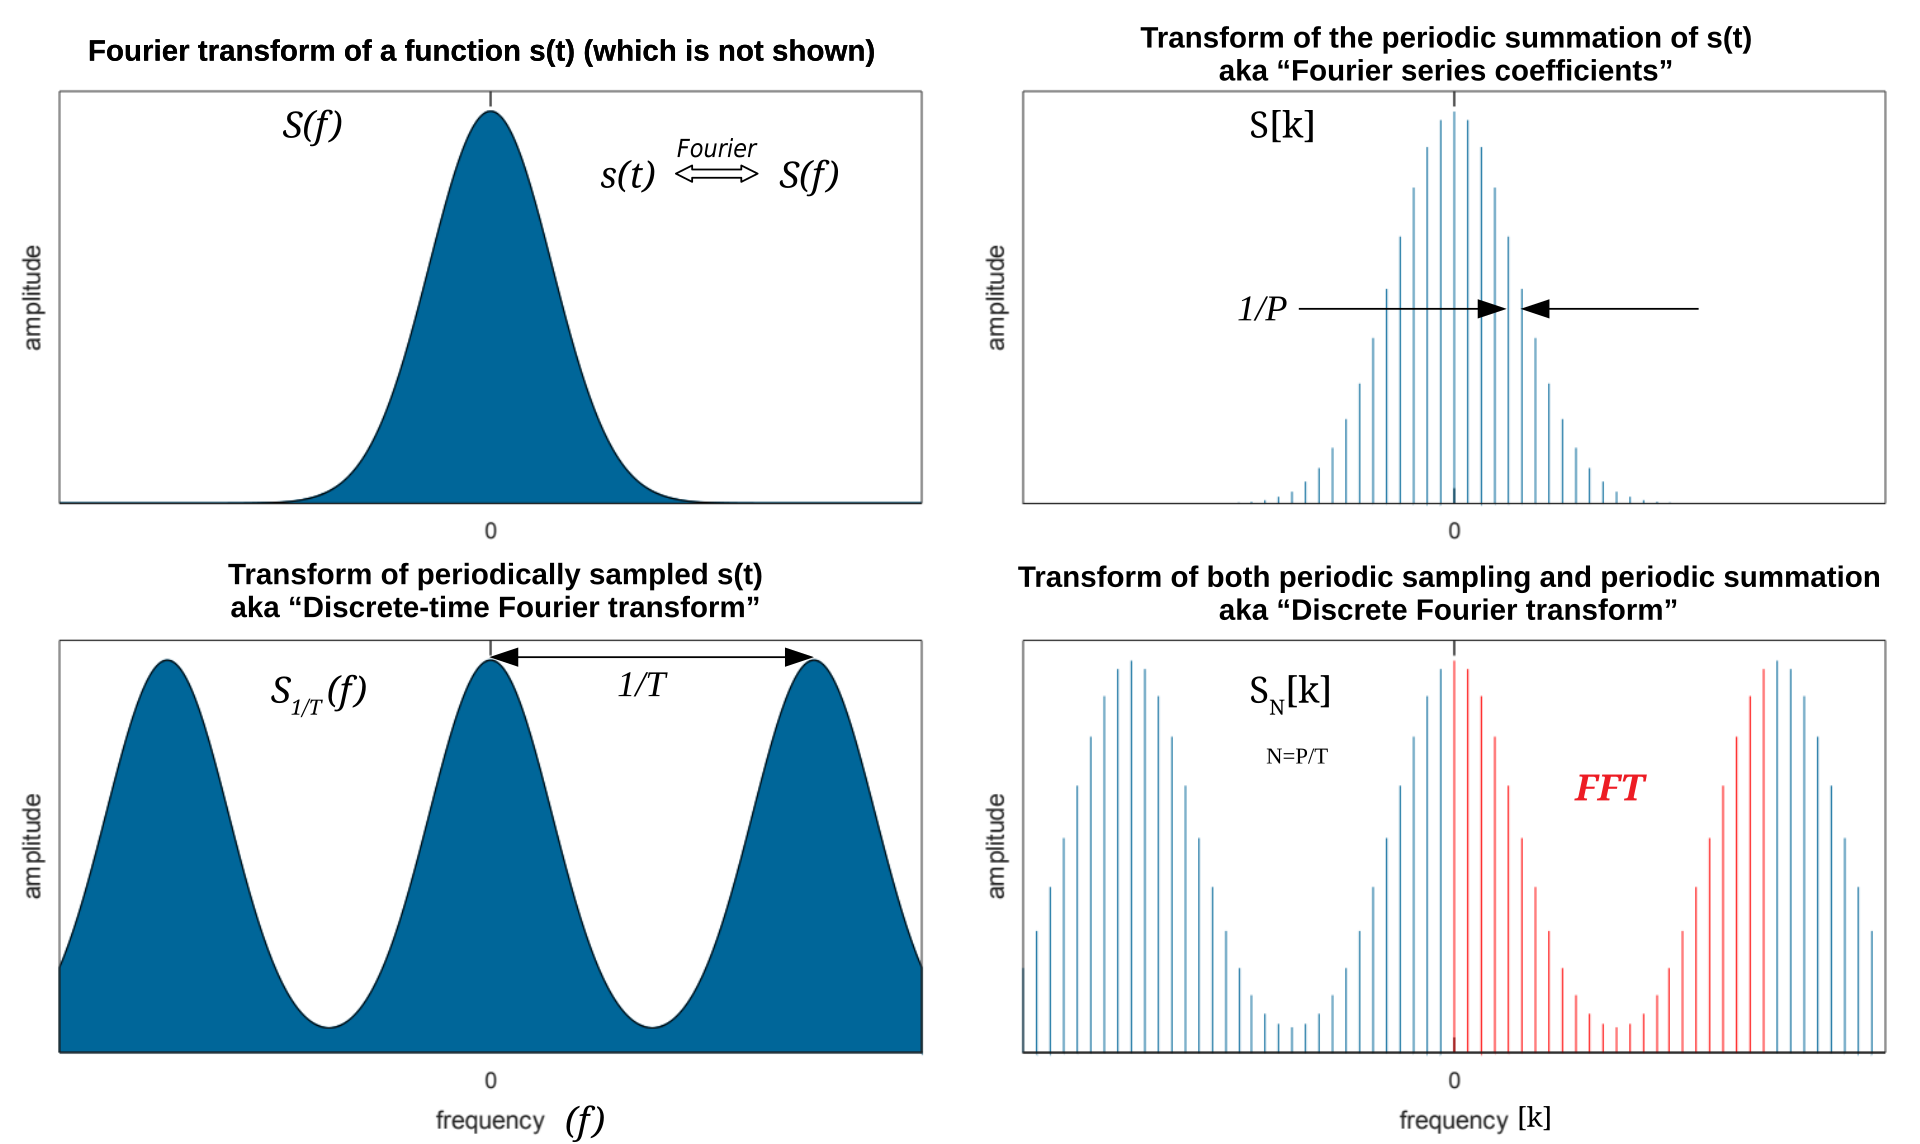
\includegraphics[width=\textwidth,height=0.8\textheight,keepaspectratio]{images/audio-nlp-eval/fourier.png}
        \caption*{Depiction of a Fourier transform. Source: Wikipedia}
    \end{figure}
\end{frame}

\subsection{Short-Time Fourier Transform (STFT)}
\begin{frame}[allowframebreaks]{Short-Time Fourier Transform (STFT)}
    \begin{itemize}
        \item STFT is a method to analyze the frequency content of a signal over time.
        \item It involves applying the Fourier Transform to short overlapping segments (frames) of the signal.
        \item The STFT provides a time-frequency representation of the signal.
    \end{itemize}
\framebreak
    \begin{itemize}
        \item \textbf{What:}
        \begin{itemize}
            \item Slide a window across the signal.
            \item Compute a DFT per frame.
        \end{itemize}

        \item \textbf{Continuous form:}
        \[
            X(t,\omega) = \int x(\tau)\, w(\tau - t)\, e^{-j \omega \tau}\, d\tau
        \]

        \item \textbf{Discrete idea:}
        \begin{itemize}
            \item DFT of windowed frame at each time step.
            \item Sources: \texttt{Wikipedia}, \texttt{courses.physics.illinois.edu}
        \end{itemize}
\framebreak
        \item \textbf{How:}
        \begin{itemize}
            \item Choose window: Hann / Hamming
            \item Frame length: e.g., 25 ms
            \item Hop: e.g., 10 ms
        \end{itemize}

        \item \textbf{Why:}
        \begin{itemize}
            \item Speech is quasi-stationary in short frames.
            \item STFT captures how spectrum changes over time.
        \end{itemize}
    \end{itemize}
    \begin{figure}
        \centering
        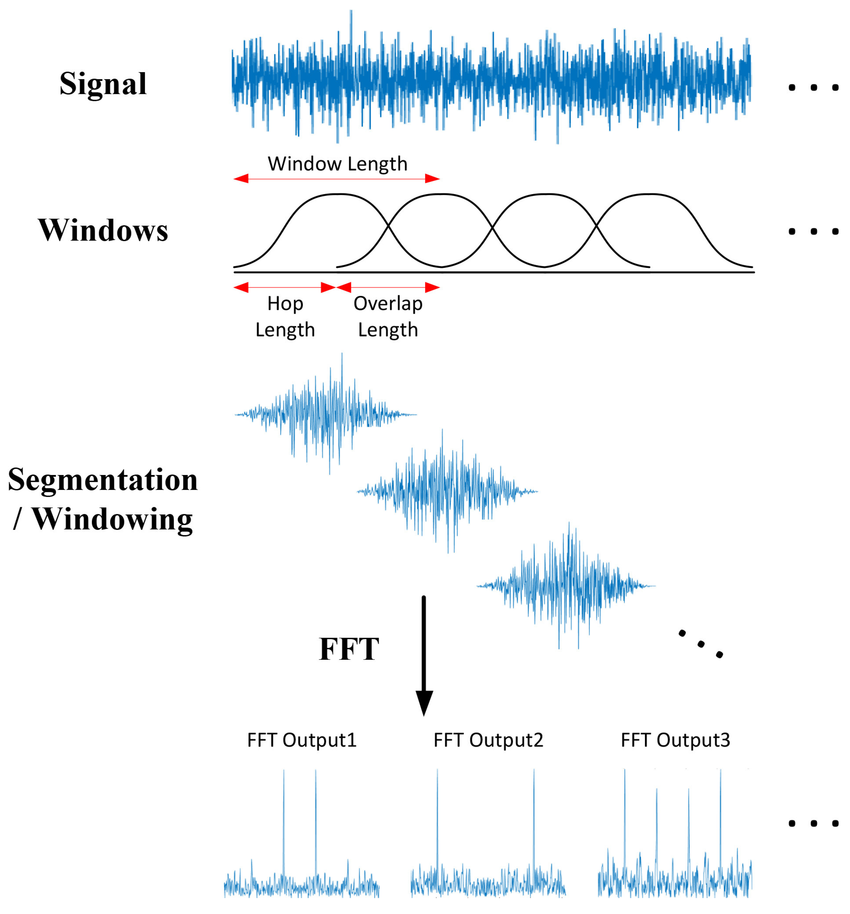
\includegraphics[width=\textwidth,height=0.8\textheight,keepaspectratio]{images/audio-nlp/stft-diagram.png}
        \caption*{STFT process: Signal divided into frames, each transformed into frequency domain.}
    \end{figure}
\framebreak
    \begin{itemize}
        \item The STFT is computed as:
        \[
            STFT(x[n]) = \sum_{m=-\infty}^{\infty} x[m] w[n-m] e^{-j2\pi f m}
        \]
        where $w[n-m]$ is a window function applied to each frame.
    \end{itemize}
\framebreak
    \begin{itemize}
        \item The result is a complex-valued matrix, where each column represents the frequency content of a frame.
        \item The magnitude of the STFT gives the amplitude of each frequency at each time step.
        \item The phase of the STFT provides information about the timing of the frequency components.
    \end{itemize}
    \begin{figure}
        \centering
        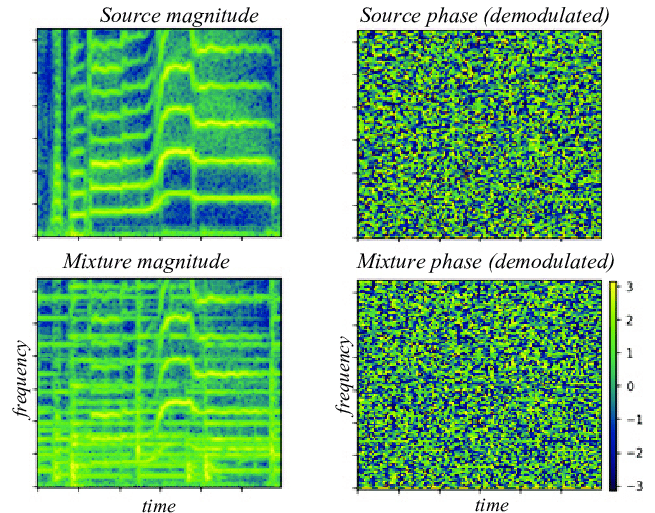
\includegraphics[width=\textwidth,height=0.75\textheight,keepaspectratio]{images/audio-nlp/stft-magnitude-phase.png}
        \caption*{Magnitude and phase of STFT: Magnitude shows amplitude, phase shows timing of frequencies.}
    \end{figure}
\end{frame}

\subsection{Spectrograms}
\begin{frame}[allowframebreaks]{Spectrograms}
    \begin{itemize}
        \item A spectrogram is a visual representation of the STFT.
        \item It displays time on the x-axis, frequency on the y-axis, and color intensity represents amplitude.
        \item Spectrograms are widely used in audio analysis, speech recognition, and music processing.
    \end{itemize}
\framebreak
    \begin{itemize}
        \item \textbf{What:}
        \begin{itemize}
            \item Heatmap of energy vs. time (x-axis) and frequency (y-axis).
            \item Color represents magnitude (often in dB).
        \end{itemize}

        \item \textbf{How:}
        \begin{itemize}
            \item Magnitude of STFT per time–frequency bin.
            \item Often log-scaled:
            \[
                20 \log_{10} |X|
            \]
        \end{itemize}

        \item \textbf{Why:}
        \begin{itemize}
            \item Visual patterns (formant tracks, harmonics, fricatives) → model-friendly features.
            \item Example: vowel formants appear as bright horizontal bands.
        \end{itemize}
    \end{itemize}
\framebreak
    \begin{figure}
        \centering
        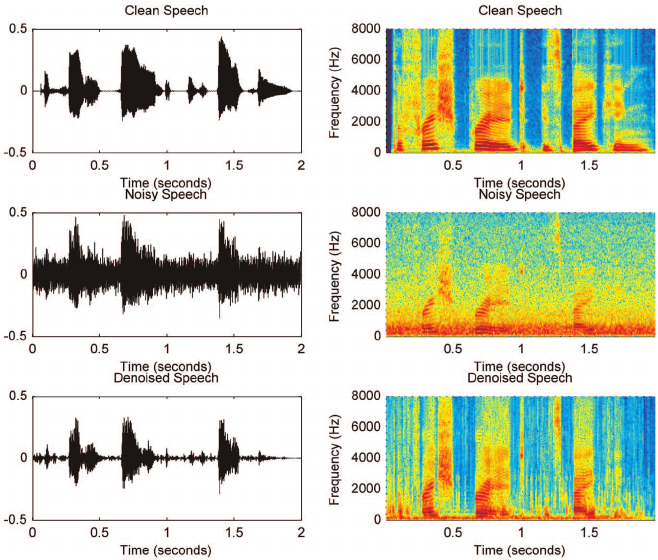
\includegraphics[width=\textwidth,height=0.8\textheight,keepaspectratio]{images/audio-nlp/spectrogram-example.png}
        \caption*{Example of a spectrogram: Time vs Frequency representation of an audio signal.}
    \end{figure}
    \begin{itemize}
        \item Spectrograms can be computed using various window functions (e.g., Hamming, Hanning) and different frame sizes.
        \item They provide insights into how the frequency content of a signal changes over time.
    \end{itemize}
    \begin{figure}
        \centering
        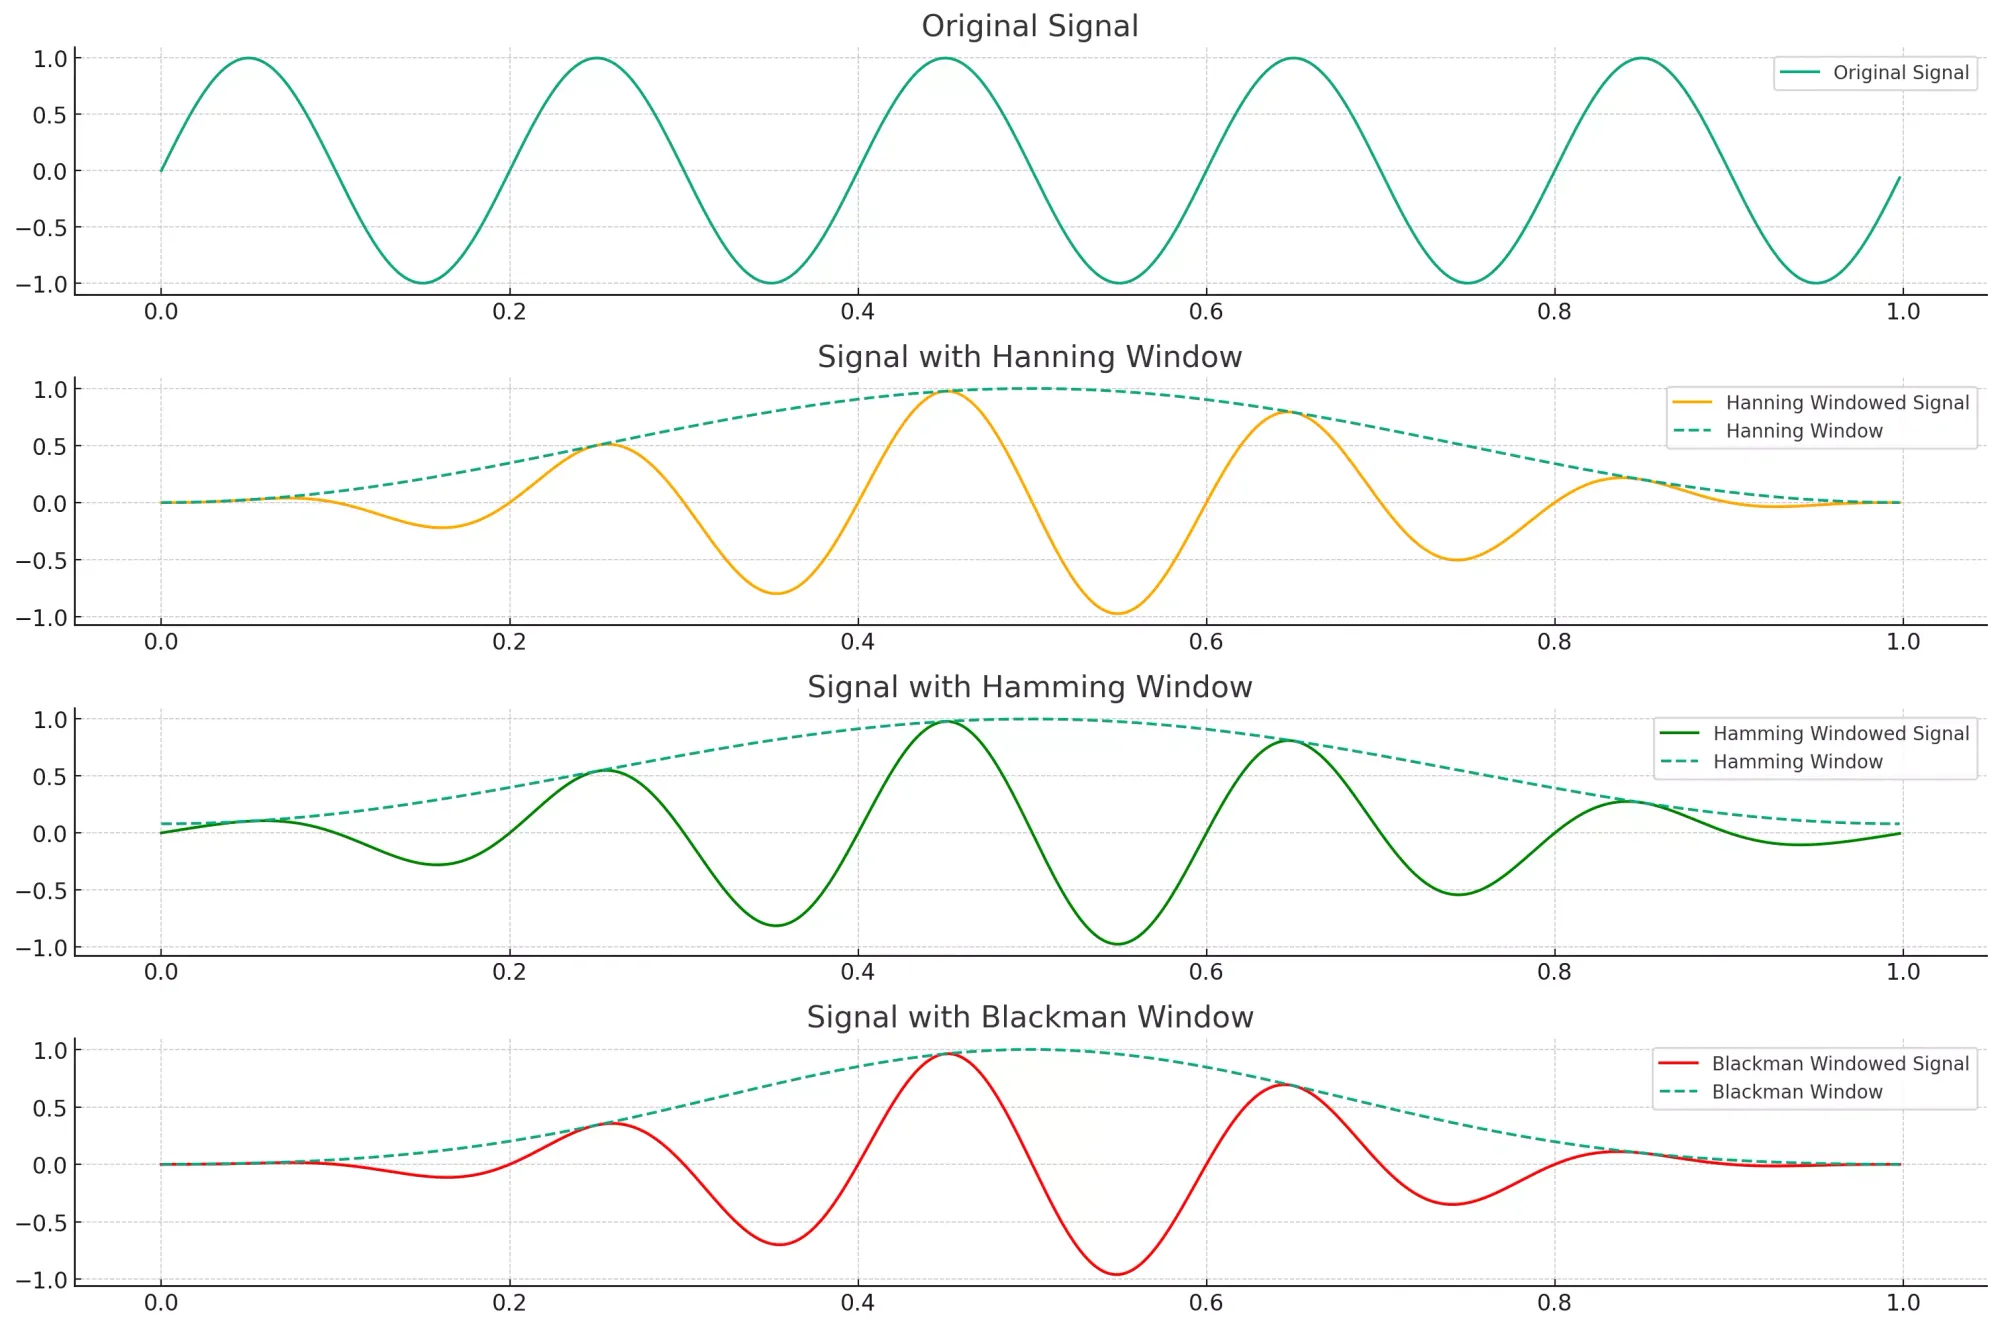
\includegraphics[width=\textwidth,height=0.75\textheight,keepaspectratio]{images/audio-nlp/spectrogram-variations.png}
        \caption*{Spectrogram variations: Different window functions and frame sizes affect the appearance of the spectrogram.}
    \end{figure}
\end{frame}